\documentclass[../../../main.tex]{subfiles}

\begin{document}
\setcounter{chapter}{11}
\chapter{Electrostatics}

\section{Coulomb's Law}

\begin{gather*}
    F=(\frac{1}{4\pi\epsilon_0})\frac{Q_1Q_2}{r^2}, \\
    \text{where } \epsilon_0= \text{permittivity of vacuum or free space}
\end{gather*}

\begin{mdframed}
    Definition: The magnitude of the electric force between two point charges is \emph{directly proportional to the product of the two charges} and \emph{inversely proportional to the square of the distance between them}.
\end{mdframed}
Given that F is inversely proportional to \(r^2\),
\begin{equation}
    F \propto \frac{1}{r^2}
\end{equation}
thus,
\begin{equation}
    \frac{F_1}{F_2}=(\frac{r_2}{r_1})^2
\end{equation}

\section{Electric Field}

\subsection{Electric Field}
\begin{mdframed}
    Definition: An electric field is a region in which an electric charge experiences a force. An electric field is represented by \textbf{electric field lines}.
\end{mdframed}

\subsection{Electric Field Strength}
\begin{mdframed}
    Definition: The electric field strength at a point is the force per unit positive charge.
\end{mdframed}

The symbol for the electric field strength is \(E\) and it's unit is \(NC^{-1}\).
The direction of \(E\) at any point is the same as the direction of the force acting on a \textbf{positive test charge} placed at that point. (\(F=E\), for positive test charge).

\bigskip

If a charge Q is placed at a point which has an electric field intensity of E, then the force F acting on the charge is given by

\begin{equation}
    F=EQ
\end{equation}

\subsubsection{Derivation of electric field strength formula at a point in an electric field produced by a point charge Q.}

\begin{figure}[h]
    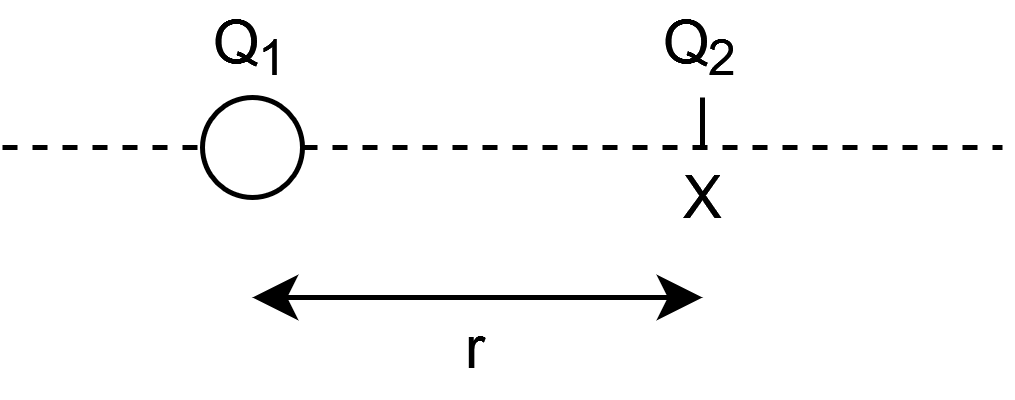
\includegraphics[]{figures/1.png}
    \centering
\end{figure}

\begin{align*}
    \text{Coulomb's Law: } F & =(\frac{1}{4\pi\epsilon_0})\frac{Q_1Q_2}{r^2}       \\
    F                        & =EQ_2                                               \\
    E                        & =\frac{F}{Q_2}                                      \\
    E                        & =\frac{Q}{4\pi\epsilon_0r^2} \text{ (Substitute F)}
\end{align*}


\end{document}